%!TEX root = ../../../adrien_gomar_phd.tex

\subsection{Numerical Setup}
We consider a simplified configuration modeling a turbomachinery 
stage. The configuration consists of a spatially 
periodic azimuthal perturbation advected downstream 
of the inlet boundary of the computational domain. 
The domain is made of two grid blocks in relative 
motion, so that the perturbation, which is steady 
in the upstream block, is seen as unsteady by the 
downstream one, and is thus representative of 
turbomachinery wakes advected across an inter-wheel interface.
The blocks are generated in cylindrical
coordinates such that the presented configuration
can be assimilated to a slice of 
a turbomachinery stage.
Without loss of generality, 
we set the rotation velocity of the upstream block to zero (stator). 
The stator is composed of $B_{stator} = 10$
"virtual" blades and the rotor by $B_{rotor} = 12$ "virtual" blades.
These are termed virtual blades as no blade is actually meshed.
This is a typical pitch ratio encountered 
in contra-rotating open rotor applications in which 
the first row contains more blades 
than the second (see Chap.~\ref{cha:cror}). Indeed, in
these applications, the number
of blades is typically smaller than classical
turbomachinery configurations. %This means that a wake
% with a given width will be seen thinner because of the bigger
% relative pitch. 

A wake is axially injected at the inlet of the
stator block following the Lakshminarayana and
Davino
similarity law defined in Eq.~\eqref{eq:similarity}.
It is schematically represented in 
Fig.~\ref{fig:rotating_blocks}.
This is thus a representative model problem of the wake shed
by an upstream row that crosses the rows interface, 
here the stator-rotor interface.

The flow is modeled through the 
Euler equations in order to avoid wake thickening
associated with viscous effects. 
The velocity is not imposed at the inlet directly
but rather through the total pressure and total enthalpy distributions:
\begin{equation}
  \label{eq:rotatingblocks_ptot}
    p_{i0} (\theta) = p_{i_{ref}} \left[1 - 
        \Delta p_i \cdot e^{
          -0.693 \left( 2 \frac{\theta}{L} \right) ^ 2}\right],
\end{equation}
\begin{equation}
  \label{eq:rotatingblocks_htot}
    h_{i0} (\theta) = h_{i_{ref}} \left[1 - 
        \Delta h_i \cdot e^{
          -0.693 \left( 2 \frac{\theta}{L} \right) ^ 2}\right],
\end{equation}
where $p_{i0}$ is the inlet total pressure, $\Delta p_i$ the total pressure
deficit in the wake,
$h_{i0}$ the inlet total enthalpy, $\Delta h_i$ the total enthalpy
deficit in the wake and $L$ the wake width.
% As the total enthalpy and total pressure deficits are not
% easy to define, they are estimated from a turbomachinery
% simulation. The idea here is to impose a distortion that
% is physical. This does not remove any generality
% to the current approach.
To impose a realistic distortion, the total pressure and
enthalpy deficits are estimated from a separate turbomachinery simulation.
This leads to $\Delta p_i = 0.025$ and 
$\Delta h_i = - 0.007$.
The negative sign is due to overturning in the wake, which
is due to velocity composition, and therefore specific to rotors.
The static pressure $p_{s_1}$ is imposed at the outlet:
\begin{equation}
    p_{s_1} = \frac{p_{ref}}{\left(1 + 
    \frac{\gamma - 1}{2} M_{ref}^2 \right) ^ {\frac{\gamma}{ \gamma - 1}}} ,
\end{equation}
the mean velocity is thus set by imposing the
target mean Mach number value $M_{ref}$.
At the azimuthal boundaries, phase-lag conditions~\cite{Erdos1977} 
are used to take into account for the space-time periodicity. %, 
% allowing to compute only a single blade passage, 
% as explained in Sec.~\ref{sec:turbomachinery_adaptation}.

Roe's scheme~\cite{Roe1981} with second-order MUSCL extrapolation 
is used for the spatial discretization of
the convective fluxes, and an implicit backward Euler scheme is used
to march the HB equations in pseudo-time.

A parametric study is carried out over the two parameters 
that influence the truncation error as defined in 
Eq.~\eqref{eq:def_truncation_error}: the number of harmonics and the wake width.
The number of harmonics used for the computations ranges from 1 to $25$.
%in order to ease 
%the post processing but 
%Note that a harmonic balance simulation represents $2N+1$ steady
%computations coupled together by a source term. This means that the
%equivalent mesh for $N=25$ computation is $(2 * 25 + 1) * 170,000 = 8,670,000$
%grid point mesh, which is large for a reduce order model problem.
The wake width $L$, that drives
Eq.~\eqref{eq:rotatingblocks_ptot} and~\eqref{eq:rotatingblocks_htot} varies
between $1\%$ and $30\%$ according to a logarithmic scale to ease 
the visualization of the results. $375$ computations are performed in total. 

Each grid block has a radial extent of five grid points \emph{i.e.} four cells. 
The azimuthal grid density in the stator and rotor blocks is kept similar
to guarantee a consistent capture of the wake on each side of the interface.
To do so, if $\Delta \theta_{cell}$ denotes the azimuthal length of a cell
at the interface, then:
\begin{equation}
   \Delta \theta_{cell} = \frac{2\pi}{B_{stator}}~\frac{1}{N_{stator}}
   = \frac{2\pi}{B_{rotor}}~\frac{1}{N_{rotor}},
   \label{eq:az_spatial_discretization_1}
\end{equation}
where $N_{stator}$ and $N_{rotor}$ are the number of cells
in the stator and the rotor, respectively. 

% This equation gives finally the relation
% between $N_{stator}$ and $N_{rotor}$ that ensures a uniform azimuthal
% grid density at the interface:
% \begin{equation}
%    12~N_{stator} = 10~N_{rotor}.
%    \label{eq:az_spatial_discretization_2}
% \end{equation}
Mesh convergence for the thinnest wake (1\% of the pitch)
is obtained with 500~cells in the azimuthal direction of
the stator which gives
600~cells for the rotor block.
30~grid points are put in the axial direction. Moreover, a constant
aspect ratio of 5 with respect to the azimuthal length of the cells is
kept, which sets the axial length of the case.
This leads to a total number of grid points of approximately 
170,000. 
Note that the memory requirement of an HB 
simulation is $2N+1$ times that of the equivalent steady case. 
An equivalent steady computation to $N=25$ would 
thus require 
$(2 \times 25 + 1) \times 170,000 = 8,670,000$ grid point mesh.
The grid used for the computations is shown in Fig.~\ref{fig:rotating_blocks}.
\begin{figure}[htb]
  \centering
  \begin{tabular}{cc}
    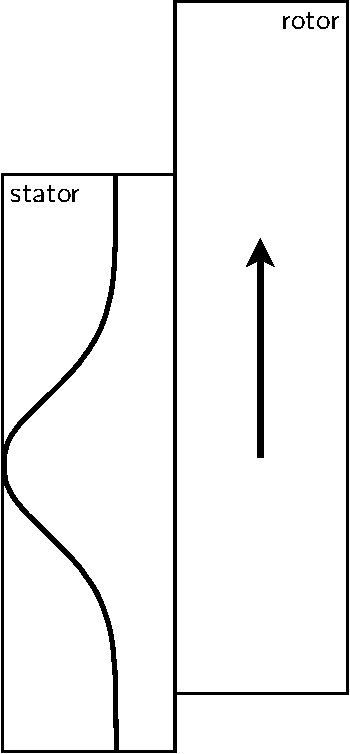
\includegraphics[height=.3\textheight]{ROTATING_BLOCKS.pdf}
    &
    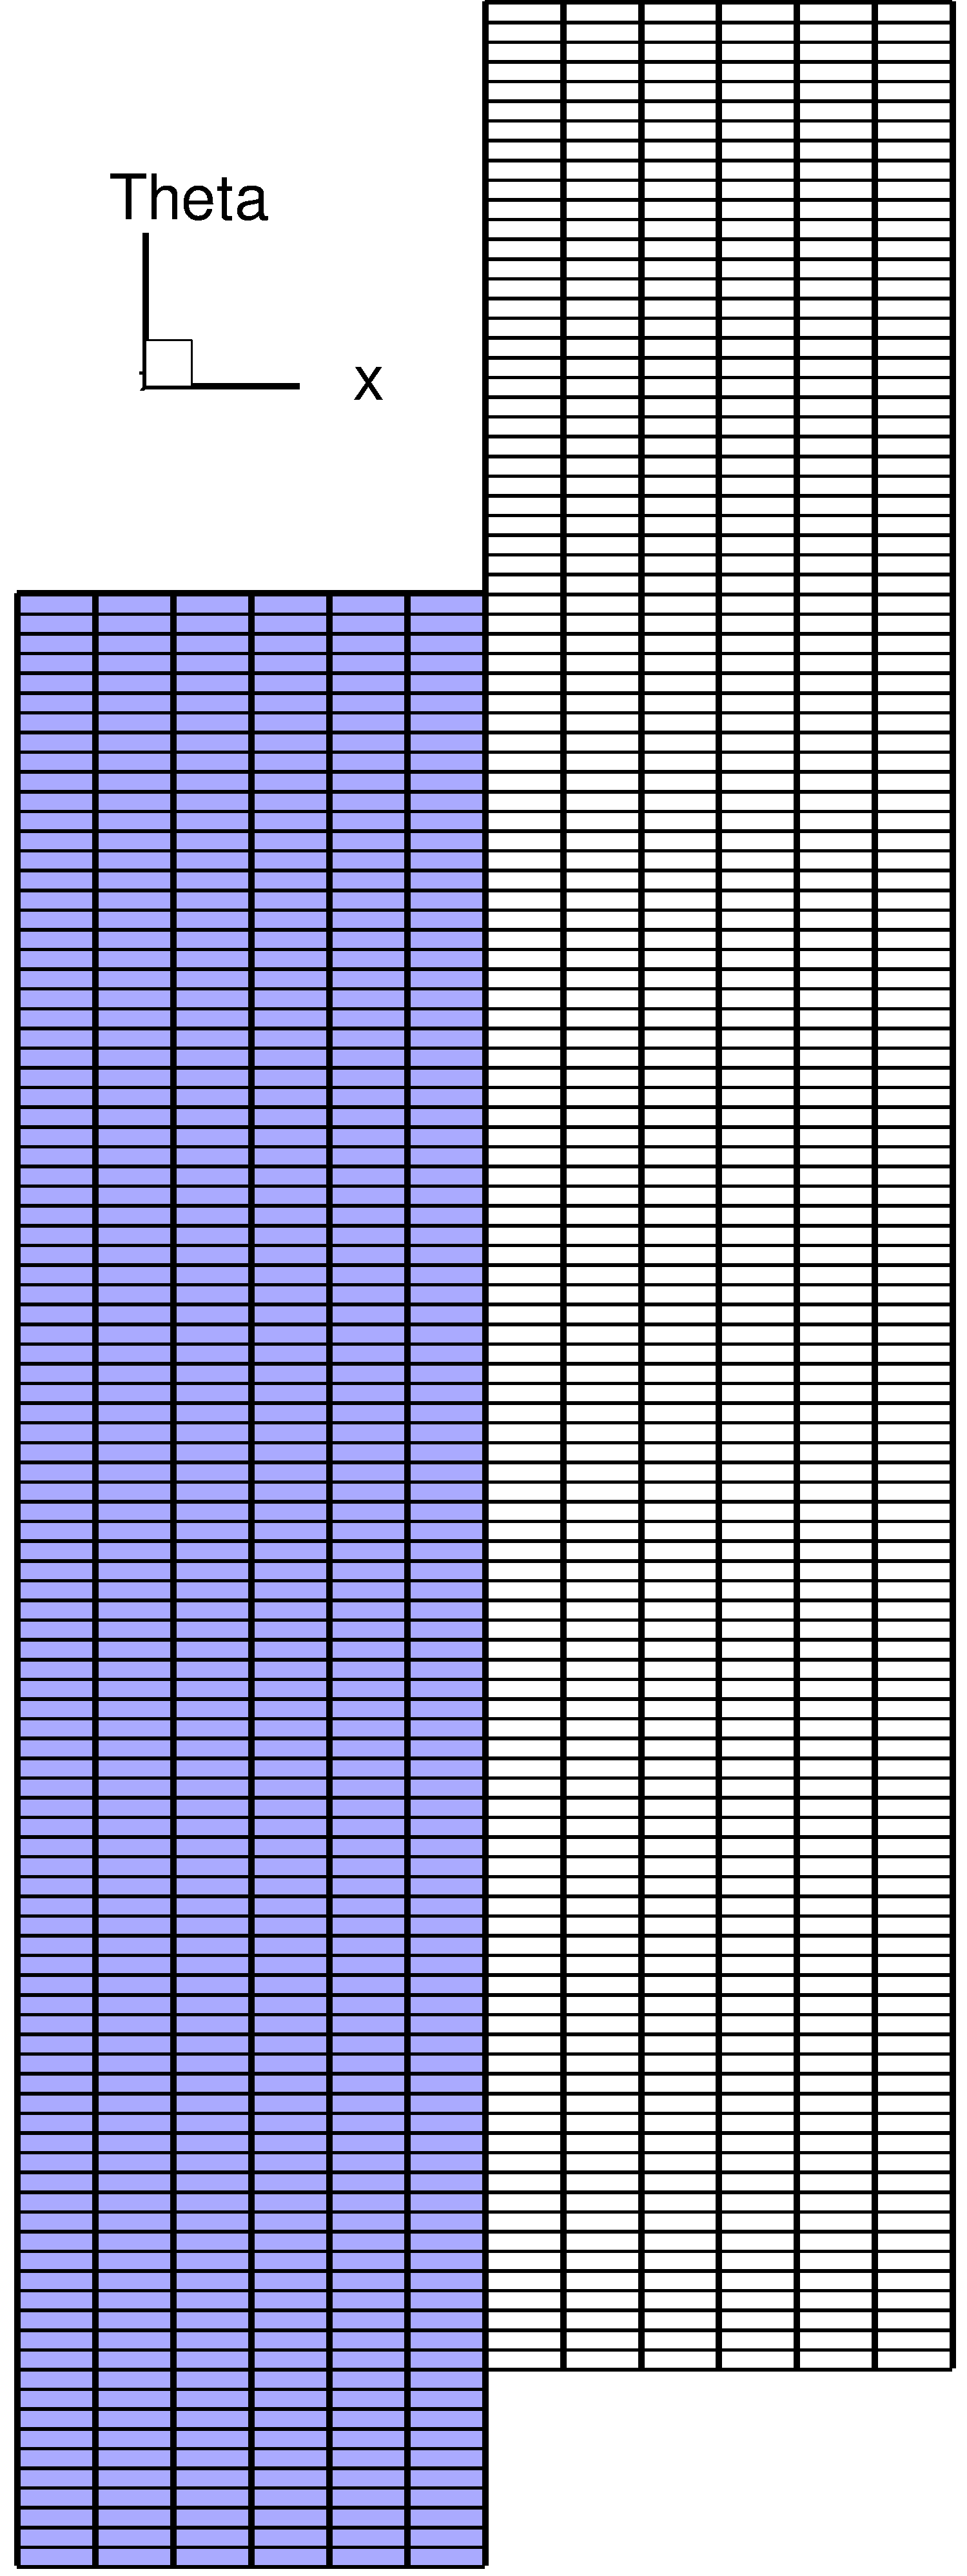
\includegraphics[height=.3\textheight]{RB_mesh_3D.png}\\
    Principle diagram 
    &
    Mesh, one out every five points
  \end{tabular}
\caption{Model turbomachinery configuration.}
\label{fig:rotating_blocks}
\end{figure}
Convergence of the iterative procedure used to solve the HB equations is achieved 
after 3,000 iterations for 
all the simulations. 